%% CLASS MANUAL FOUND IN http://blog.poormansmath.net/latex-class-for-lecture-notes/ %%
%% CLASS AUTHOR Stefano Maggiolo %%

%%%%%%%%%%%%%%%  TITLE PAGE  %%%%%%%%%%%%%%%%%%%
\documentclass[english,course]{Notes}
\title{Web Application Development}
\subject{CS - Web Development}
\author{Joao Almeida-Domingues}
\email{2334590D@student.gla.ac.uk}
\speaker{Dr. Alistair Morrison}
\date{15}{01}{2020}
\dateend{25}{03}{2020}
\place{University of Glasgow}

\graphicspath{{assets/}}
%%%%%%%%%%%% BIB CONFIG %%%%%%%%%%%%%%%
\usepackage[backend=biber, style=reading,
citestyle=numeric]{biblatex}

\bibliography{wad} %add bib file name

%%%%%%%%%%% LAYOUT  %%%%%%%%%%%%%%%

\renewcommand{\abstractname}{\vspace{3\baselineskip}} %hack to remove abstract
\lstset{
  basicstyle=\ttfamily,
  columns=fullflexible,
  frame=single,
  breaklines=true
 }

%%%%%%%%%%%%%%%%%%%%%%%%%%%%%%%%

%%%%%%%%%%%%%% KEEP HERE (conflict when in class) %%%%%%%%%%%%%%%%%%%%

 %%%%%MATRICES

    \let\mat=\spalignmat
    \let\amat=\spalignaugmat
    \let\vec=\spalignvector

%%%%%% row ops
    \newcommand\ro[2]{\xrightarrow[#2]{#1}}
%%%%%%%%%%%%%%%%%%%%%%%%%%%%%%%%%%%%%%%%%%%%%%%%%%%%%

%%%%%%%%%%%%%  PACKAGES (NOT INCLUDED IN CLASS) %%%%%%%%%%%%%%
\usepackage[delims={[]}]{spalign}
\usepackage{multicol}
%%%%%%%%%%%%%%%% ALGORITHM TEMPLATE %%%%%%%%%%%%%%%%%%%%

%\begin{algorithm}[H]
%\SetAlgoLined\KwData{this text}
%\KwResult{how to write algorithm with \LaTeX2e }initialization\;
%\While{not at end of this document}
%	{read current\;\eIf{understand}{go to next section\;current section becomes this one\;}{go back to the beginning of current section\;}}
%	\caption{How to write algorithms}
%\end{algorithm}

%%%%%%%%%%%%%%%%%%%%%%%%%%%%%%%%%%%%%%%%%%%%%%%%%%%%%

\begin{document}

%%%%%%%%%%%%%%  DISCLAIMER  %%%%%%%%%%%%%%%%%%%%%

\begin{abstract}
	\par{These lecture notes were collated by me from a mixture of sources , the two main sources being the lecture notes provided by the lecturer and the
content presented in-lecture. All other referenced material (if used) can be found in the \ita{Bibliography} and \ita{References} sections.}
	\par{The primary goal of these notes is to function as a succinct but comprehensive revision aid, hence if you came by them via a search engine , please note
that they're not intended to be a reflection of the quality of the materials referenced or the content lectured.}
	\par{Lastly, with regards to formatting, the pdf doc was typeset in \LaTeX , using a modified version of Stefano Maggiolo's \href{http://blog.poormansmath.net/
latex-class-for-lecture-notes/}{\underline{\textcolor{blue}{class}}}}
\end{abstract}
\newpage

%%%%%%%%%%%%% LECTURES %%%%%%%%%%%%%%%%%%%%%%%

%\section{Introduction}

\subsection{ILOs - Fundamentals}

\par{The goal of the course will be to deepen your understanding of the fundamental
principle and techniques in computer systems, such as:}
\begin{itemize}
	\item Memory and computation as fundamental resources of computing
	\item Representation of data structures in memory and the role of data types
	\item Techniques for management of computational resources
	\item Reasoning about concurrent systems
\end{itemize}


\subsection{Systems vs Application Software}

\par{We contrast system software with application software. System software can be seen as
low-level software, i.e it usually concerns itself with interacting with the machine directly or
very close to the metal whilst providing abstractions for application software}
\par{There are constraints which come with the nature of system software, such as fast
execution time, low memory consumption or low energy usage. Because high-level, managed languages are usually
highly abstract, it is almost impossible to build software which abides by these constraints, hence
one uses system programming languages like \texttt{C} which provide the programmer with more fine
grained control over how their program will execute}


\subsection{History}

\par{In the 1950s the distinction between these two types of software was nonexisting.
Machines were very much purposely built to run certain applications and a single executing
application would use the entire machine. \ita{Grace Hopper} was responsible for writing one of the
first compilers which turned human readable code into machine code.}

\par{Until the 1970s system software was always written in a processor specific assembly
language, which meant that for each new processor a systems programmer would need to rewrite the
same program in a different assembly language. In the 1970s \ita{Dennis Ritchie} and \ita{Ken Thompson} , while trying to port \texttt{UNIX} between two machines, invented \texttt{C} as a
\ita{portable, imperative} language which supported \ita{structured programming.}}

\par{In the 1980s, \ita{Stroustroup} came up with \texttt{C++} primarily so that he could
automate certain tasks which have to be done manually in C.}

\par{Until the 2010s the focus very much shifted towards the development of high-level, managed
languages however, the emergency of mobile devices rekindled the interested in new systems languages such as \texttt{Swift} and \texttt{Rust} which permit the devices to not waste their already scarce resources in tasks such as garbage collection}

\section{C - Introduction}

\key{introduction to C}{fundamental features}{differences}{strong
typin}{lexical scope}{lifetime of variables}{call by value}{declarations and definitions}{compiler
errors and warnings}{data representation in memory}{data types}

\subsection{A tale of two languages}

\par{In order to illustrate the advantages of C over managed languages take the following programs}

\noindent\begin{minipage}[t]{.45\textwidth}
	\begin{lstlisting}[language=python,]

	x = 41
	x = x + 1
	\end{lstlisting}
	\end{minipage}
\noindent\begin{minipage}[t]{.45\textwidth}
	\begin{lstlisting}[language=C,]
int main() {
	int x = 41;
	x = x + 1;
}
	\end{lstlisting}
\end{minipage}


\rem{Java syntax was heavily borrowed from C. Programs differ in how they are executed and on how memory is organised}

\par{The size (in memory) of \texttt{x} in Python is dependent on the architecture, in this computer for example is about 28B, whilst in C is just 4B. Why? Given the dynamic nature of python, its C implementation uses a descriptor object which stores the alongside the value which significantly increases the memory requirements. In C integers are usually 4B and that's all you need to represent \texttt{x} in memory }

\par{What about the number of instructions? That's even harder to know in python, because for example each operation must type-check first, then it must also check that addition is a valid operation and it represents all of that in some structure in the CPU. In C however, we know that only 3 instructions are required, 1 \texttt{add} and 2 \texttt{mov}.}

\rem{This level of fine-grained control allows us to confidently reason about the execution behaviour and performance of a program}

\subsection{Compiling}

\par{The compiling of code is the act of transforming the source code of a program into an executable file which can be run by the OS. There are two kinds of source files in C:}

\begin{itemize}
	\item \href{https://gcc.gnu.org/onlinedocs/cpp/Header-Files.html}{Header Files} : a file containing C declarations and macro definitions to be shared between several source files. Its contents can be requested in a program by including it, with the C preprocessing \textit{directive} \texttt{\#include}.  It is conventional to end file names with \texttt{.h}

	\item Compilation Units : These are \texttt{.c} files whose directives are replaced by the contents of the header files. Each file is compiled separately to keep compilation times short
\end{itemize}

\par{The compilation process can be split into 3/4 main steps:}

\begin{itemize}\item{Preprocessor : During the preprocessing stage the preprocessor will look at the source code and replace all directives and macros with the contents of their corresponding files. For examples \texttt{\#include <stdio.h>} will copy the contents of the I/O library \texttt{stdio.h}}

	\rem{To see an example of the output run \texttt{gcc -E}}

	
	\item{Compiler \& Assembler : The compiler transforms the preprocessed code into assembly code which in turn are turned into \textit{object} files \texttt{.o} (almost executable) by the assembler}

	\item{Linker : The linker will then find, for each name appearing in the object code, the address that was eventually assigned to that name, make the substitution, and produce a true single binary executable in which all names have been replaced by addresses}
\end{itemize}

\rem{You can use constants by using the \texttt{\#define} compiler directive which will essentially
replace every instance of the named variable with the actual value at preprocessing stage}


\subsubsection{Warnings \& Errors}

\par{Compiling errors mean that it is impossible to translate the program into an executable.
Warnings on the other end indicate that there is something and unusual in the code which will most
likely result in a runtime error. Occasionally one might want to keep the piece of code which threw the warning , in that case make sure to make that
clear in your code.\mymarginpar{For the coursework make sure that
to submit code which compiles without warnings}} 

\par{The compiler and the linker will throw different kinds of errors, being able to identify which is which helps with debugging. For example, it is possible to convert a program into object code which has a call to an undefined function this will just throw a warning. However, when running the linker an error will be thrown and an executable won't be created.}

\rem{\texttt{-Werror} turns all warnings into errors, the \texttt{-Wall} flag enables most compiler
warnings}








%\section{Django - Introduction}

\par{Django is a web framework which makes building web apps simpler and faster,
by providing:}

\begin{enumerate}
	\item[]{a division between logic and presentation components}
	\item[]{auto-generation of web admin}
	\item[]{many APIs for common tasks}
	\item[]{extra URL mapping control \mymarginpar{URL-Django-HTML vs URL-HTML}}
\end{enumerate}

\subsection{Design Philosophy}

	\par{Django follows the \ita{loose coupling} principle, which states that
different layers of the app should not know about each other's details ; and the
\ita{DRY} principle which states that \ita{"Every piece of knowledge must have a single, unambiguous, authoritative
representation within a system"}, i.e one should know exactly where to lookup
required data without having to repeat it in logically separate modules}

\subsection{Essential (pre-packaged) Modules}

\begin{itemize}
	\item[]{Create Read Update Delete Admin Interface}
	\item[]{Authorization Systems}
	\item[]{Form, Session Handling}
	\item[]{Syndication Awareness (e.g. RSS)}
	\item[]{Caching}
	\item[]{Internationalization}
\end{itemize}

\subsection{MVT}

\defn{ORM}{a programming technique for converting data of different types using
OO concepts and languages}

\par{Django uses a variant of the
\href{https://blog.codinghorror.com/understanding-model-view-controller/}{MVC}
design pattern - \ita{MVT}.The Model-View-Template is a \ita{data-driven} framework which separates
an app into the following logical units}

\begin{enumerate}
	\item{\textbf{Models : } is an abstraction of the database, where data
structures are represented via python objects}

	\par{This abstraction is achieved via \ita{Object Relational Mapping} ,
where one can query the database via the usual object dot access notation, and
Django in the background, converts both the objects and our queries into valid
SQL (or whatever DB language the project is using)}

	\item{\textbf{Views : } provide both the representation logic and app logic.
It's here that one handles HTTP requests/responses via response objects. It
is also here than one can query data via
the models' API, where a template populated with results is returned for
presenting}
	\item{\textbf{Templates : } provide the presentation layout (decoupled from
the data), composed of
static HTML, with the possibility of using the \ita{django template language} to
include some dynamic elements}
\end{enumerate}

	\begin{figure}[H]
		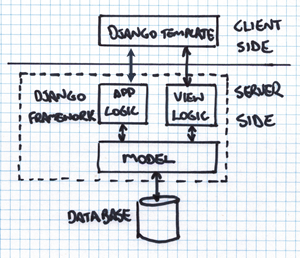
\includegraphics{mvt.png}
		\caption{\href{https://djangobook.com/mdj2-django-structure/}{Django
MVT}}
	\end{figure}

 \rem{Views are not queried directly via the client, instead the urls.py file
allows for finer control, pairing a given URL (or URL pattern) to a certain
view.}



\section{AJAX}

\par{AJAX stands for \ita{Asynchronous Javascript and XML}, and represents a set of key technologies which when used together allow web applications to be updated without needing to reload each time. With AJAX, web applications can send and retrieve data from a server asynchronously effectively decoupling the data interchange layer from the presentation layer}

\rem{nowadays is far more common to use JSON instead of XML}


	\subsection{Asynchronicity}


		\par{The key element behind AJAX is the \texttt{XmlHttpRequest Object}, which is just a \texttt{DOM} object, with the special property of being able to exchange data with the server behind the scenes.}

		\par{In contrast with classical webpages, the JS engine handles requests and is then able to update only the targetted parts of the web app which need updating. Unlike forms, or links the \texttt{XmlHttpRequest Object} does not block script execution the JS keeps running in the background, hence the asynchronous nature of the requests.}


		\lstinputlisting[]{assets/ajax.js}


	\subsubsection{Summary}

		\begin{enumerate}
			\item An event occurs
			\item An \texttt{XmlHttpRequest Object} is created by JS
			\item An HTTP request is sent to the server
			\item The server processes the request
			\item The server sends back the response
			\item The JS engine processes the response
			\item The DOM is manipulated appropriately by the JS
		\end{enumerate}


	\subsection{The \texttt{XmlHttpRequest Object}}

		\url{https://www.w3schools.com/xml/ajax_xmlhttprequest_create.asp}


	\subsection{Callbacks}

		\par{When performing multiple tasks using AJAX, there should be a main function which sets the request object and then there should be different \ita{callback} functions for each task.}

		\rem{the main function call should contain the \texttt{URL} and the function to call when the response is ready}

		\lstinputlisting[language=HTML]{assets/ajax_callback.html}






%%%%%%%%%%%%%%  BIBLIOGRAPHY  %%%%%%%%%%%%%%%%%%%
\newpage
\nocite{*}
\printbibliography

%%%%%%%%%%%%%%%%%%%%%%%%%%%%%%%%%%%%%%%%%%

\end{document}
